\documentclass{ctexart}

\usepackage{ctex}
\usepackage{tikz}
\usetikzlibrary{calc,positioning,shapes.geometric}
\usepackage{url}
\usepackage{graphicx}
\usepackage{float}
\usepackage{xcolor}
\usepackage{color}
\usepackage{amsmath}
\usepackage{amsthm}
\usepackage{amssymb}
\usepackage{mathrsfs}
\usepackage{caption}
\usepackage{subfigure}
\usepackage{framed}
\usepackage{booktabs}
\usepackage{makecell}
\usepackage{geometry}
\usepackage{wrapfig}
\usepackage{abstract}
\usepackage{algorithmicx}
\usepackage[ruled]{algorithm}
\usepackage{algpseudocode}
\usepackage{setspace}
\usepackage{bm}
\usepackage{cite}
\usepackage{array}
\usepackage{textcomp}
\usepackage{listings}

\definecolor{shadecolor}{rgb}{0.93,0.93,0.93}
\usepackage{geometry}
\geometry{right=2.5cm,left=2.5cm}

\newtheorem{theorem}{定理}

\pagenumbering{arabic}

\begin{document}
\begin{sloppypar}
\title{\vspace{-3cm} \textbf{数值分析项目作业报告}}
\author{刘陈若\;$3200104872$\\信息与计算科学2001}
\date{}

\maketitle

\section{程序编译和运行说明}
本次项目作业采用Makefile文件对编译进行统一管理。具体地,在Makefile所在目录下输入\verb|make|
即可完成编译,得到\verb|report.pdf|,problem\verb|B|的可执行文件\verb|B|,problem\verb|C|和problem\verb|D|共同的可执行文件\verb|CD|,以及problem\verb|E|的可执行文件\verb|E|。分别对其进行运行,即可得到各小题的程序运行结果。

需要说明两点:首先,本项目作业使用eigen3进行线性方程组求解,并使用json file进行参数输入,它们分别以\verb|#include <eigen3/Eigen/...>|和\verb|#include <jsoncpp/json/json.h>|的形式被调用,因此在编译时需要保持相应的文件关系;其次,报告使用json file进行参数输入时,参数的含义将在下文中详细给出,以便完成报告中的所有测试。

\section{程序运行结果及简要分析}
\subsection{spline.h 设计思路}
在\verb|spline.h|头文件中,一共设计了\verb|Function|,\verb|Interpolation|两个基类,派生出不同的class以满足项目要求。以下将分别展开设计思路叙述。
\subsubsection{class Function}
\verb|Function|类一共设计了\verb|operator()|(括号重载),\verb|diff|和\verb|diff_2|三个虚函数,用于返回给定函数的值以及一二阶导数的值。对于无需求导数的函数,其导数默认为0。总体而言,\verb|Function|类主要功能有三:存储待样条插值的函数,存储B样条基函数以及存储ppForm插值后得到的多项式函数。

$\bullet \;$\verb|class Discrete_function|:对于待样条插值的函数,若给出了函数的解析表达式,直接派生相应的函数类即可;若没有给出函数的解析表达式,也就是以离散点集给出的函数,还设计了派生类\verb|class Discrete_function|进行相应的处理。由此,有无显示表达式的函数得到了形式上的统一,这在曲线拟合中起到了重要作用。

$\bullet \;$\verb|class B_spline|:对于B样条基函数,设计了派生类\verb|class B_spline|,利用\textbf{Definition 3.23}递归返回样条基函数的值:如果阶数为1则直接利用解析表达式返回值,否则利用课本式(3.30)递归。

$\bullet \;$\verb|class Polynomial|:由于进行ppForm插值后得到的是许多个分段多项式,因此还设计了派生类\verb|class Polynomial|,存储形如$a_0+a_1(x-a)+\dots+a_n(x-a)^n$的多项式(多项式的“分段”任务将在之后的interpolation类中完成)。
\subsubsection{class Interpolation}
\verb|Interpolation|类主要功能是为了实现基于ppForm和B样条法的线性样条及$\mathbb{S}^2_3$样条(以下简称三次样条)插值,并基于此完成曲线插值。\verb|Interpolation|类一共设计了\verb|solve|和\verb|operator()|(括号重载)两个虚函数,分别用于插值算法求解以及返回求解后插值函数在某一点处的值。

$\bullet \;$\verb|class Bspline_interpolation|:对于B样条插值,设计了该派生类以支持线性样条和三次样条插值,其中三次样条插值支持complete cubic spline(以下简称CCS),cubic spline with specified second derivatives at its end points(以下简称CS-SSD)和natural cubic spline(以下简称NCS)三种边界条件。

给定不一定等间距的插值点$t_1,\dots,t_N$,待插值函数$f(x)$,以及插值阶数和边界条件,\verb|solve|函数利用eigen3的稀疏矩阵LU分解求解线性方程组$Ax = b$得到B样条基函数的对应系数$x$从而求得插值函数$S(x)$。经过数学推导,以下给出各种情况对应的矩阵$A$和向量$b$的具体表达式。由于推导过程非常繁琐,此处只给出最终结果。

对于线性样条,在添加额外的插值点$t_0,t_{N+1}$(理论上是任意的,本算法采用等间隔添加,即使得$t_1-t_0=t_2-t_1$,$t_{N+1}-t_{N} = t_{N}-t_{N-1}$)后可设
\begin{equation}
    S(x) = \sum^N_{i=1}a_iB^1_i(x),\quad x^T = [a_1,\dots,a_N],
\end{equation}
则有
\begin{equation}
    A = I_N,\quad b^T = [f(t_1),\dots,f(t_N)].
\end{equation}

对于三次样条,在添加额外的插值点$t_{-2}$至$t_0$,$t_{N+1}$至$t_{N+3}$(方法同上)后可设
\begin{equation}
    S(x) = \sum^N_{i=-1}a_iB^3_i(x),\quad x^T = [a_{-1},\dots,a_N],
\end{equation}
并记
$$
A = 
\begin{bmatrix}
    m_{1,1} & -m_{1,1}-m_{1,3}& m_{1,3} & & \\
    B^3_{-1}(t_1) & B^3_{0}(t_1) & B^3_{1}(t_1) & &\\
    & \ddots & \ddots & \ddots &\\
    & & B^3_{N-2}(t_N) & B^3_{N-1}(t_N) & B^3_{N}(t_N) \\
    & & m_{N+2,N} & -m_{N+2,N}-m_{N+2,N+2} & m_{N+2,N+2}
\end{bmatrix}
, \quad b = 
\begin{bmatrix}
    b_1 \\
    f(t_1) \\
    \vdots \\
    f(t_N) \\
    b_{N+2} \\
\end{bmatrix}
$$
则对CCS有$b_1 = f'(t_1)$,$b_{N+2} = f'(t_N)$,
\begin{equation}
    m_{1,1} = -\frac{3B^2_{0}(t_1)}{t_2 - t_{-1}},\quad m_{1,3} = \frac{3B^2_{1}(t_1)}{t_3 - t_{0}},\quad m_{N+2,N} = -\frac{3B^2_{N-1}(t_N)}{t_{N+1} - t_{N-2}},\quad m_{N+2,N+2} = \frac{3B^2_{N}(t_N)}{t_{N+2} - t_{N-1}};
\end{equation}
对CS-SSD有$b_1 = f^{''}(t_1)$,$b_{N+2} = f^{''}(t_N)$,
\begin{equation}
\begin{split}
    &m_{1,1} = \frac{6}{(t_2 - t_{-1})(t_2 - t_{0})},\quad m_{1,3} = \frac{6}{(t_3 - t_{0})(t_2 - t_{0})},\\
    &m_{N+2,N} = \frac{6}{(t_{N+1} - t_{N-2})(t_{N+1} - t_{N-1})},\quad m_{N+2,N+2} = \frac{6}{(t_{N+2} - t_{N-1})(t_{N+1} - t_{N-1})};
\end{split}
\end{equation}
对NCS有$b_1 = 0$,$b_{N+2} = 0$,
\begin{equation}
\begin{split}
    &m_{1,1} = \frac{6}{(t_2 - t_{-1})(t_2 - t_{0})},\quad m_{1,3} = \frac{6}{(t_3 - t_{0})(t_2 - t_{0})},\\
    &m_{N+2,N} = \frac{6}{(t_{N+1} - t_{N-2})(t_{N+1} - t_{N-1})},\quad m_{N+2,N+2} = \frac{6}{(t_{N+2} - t_{N-1})(t_{N+1} - t_{N-1})}.
\end{split}
\end{equation}
由此可知,对于任一种情况此时的$A$和$b$都是已知的,从而解得对应的$x$,进而唯一确定插值函数$S$完成插值过程。

进一步,\verb|operator()|可以返回插值函数$S$在任一点的函数值,如有需要,\verb|Get_coef|函数则用于返回系数$x$(一般不使用)。需要注意的是,本算法使用\verb|std::vector<B_spline>|存储全体B样条基函数至vector中以避免重复计算,并且在\verb|operator()|函数中仅考虑函数值不为0的部分基函数进行累加以提高算法运算效率。

$\bullet \;$\verb|class ppForm_interpolation|:对于ppForm样条插值,设计了该派生类以支持线性样条和三次样条插值,其中三次样条插值同样支持CCS,CS-SSD和NCS三种边界条件。

给定不一定等间距的插值点$t_1,\dots,t_N$,待插值函数$f(x)$,以及插值阶数和边界条件,设插值函数为$S(x)$,并记$p_i(x)=s|_{[t_i,t_{i+1}]}$,则对于线性样条插值,\verb|solve|函数直接求解得到
\begin{equation}
    p_i(x)=\frac{f(t_{i+1})-f(t_i)}{t_{i+1}-t_i}x + f(t_{i+1})-t_i\frac{f(t_{i+1})-f(t_i)}{t_{i+1}-t_i}.
\end{equation}
对于三次样条插值,\verb|solve|函数利用eigen3的稀疏矩阵LU分解求解类似\textbf{Theorem 3.7}的线性方程组$Ax = b$得插值点处的导数值$x$从而求得插值函数$S(x)$。经过数学推导,以下给出不同边界条件对应的矩阵$A$和向量$b$的具体表达式。

沿用\textbf{Lemma 3.3}的记号,设$x^T = [m_{1},\dots,m_N]$,那么对CCS有
$$
A = 
\begin{bmatrix}
    1 & & & & \\
    \lambda_2 & 2 & \mu_2 & &\\
    & \ddots & \ddots & \ddots &\\
    & & \lambda_{N-1} & 2 & \mu_{N-1} \\
    & & & & 1
\end{bmatrix}
, \quad b = 
\begin{bmatrix}
    f'(t_1) \\
    3\mu_2f[t_2,t_3]+3\lambda_2f[t_1,t_2] \\
    \vdots \\
    3\mu_{N-1}f[t_{N-1},t_{N}]+3\lambda_{N-1}f[t_{N-2},t_{N-1}] \\
    f'(t_N) 
\end{bmatrix}
;
$$
对CS-SSD有
$$
A = 
\begin{bmatrix}
    4 & 2 & & & \\
    \lambda_2 & 2 & \mu_2 & &\\
    & \ddots & \ddots & \ddots &\\
    & & \lambda_{N-1} & 2 & \mu_{N-1} \\
    & & & 2 & 4
\end{bmatrix}
, \quad b = 
\begin{bmatrix}
    6f[t_1,t_2] - f^{''}(t_1)(t_2-t_1)\\
    3\mu_2f[t_2,t_3]+3\lambda_2f[t_1,t_2] \\
    \vdots \\
    3\mu_{N-1}f[t_{N-1},t_{N}]+3\lambda_{N-1}f[t_{N-2},t_{N-1}] \\
    6f[t_{N-1},t_{N}] + f^{''}(t_N)(t_N-t_{N-1}) 
\end{bmatrix}
;
$$
对NCS有
$$
A = 
\begin{bmatrix}
    4 & 2 & & & \\
    \lambda_2 & 2 & \mu_2 & &\\
    & \ddots & \ddots & \ddots &\\
    & & \lambda_{N-1} & 2 & \mu_{N-1} \\
    & & & 2 & 4
\end{bmatrix}
, \quad b = 
\begin{bmatrix}
    6f[t_1,t_2]\\
    3\mu_2f[t_2,t_3]+3\lambda_2f[t_1,t_2] \\
    \vdots \\
    3\mu_{N-1}f[t_{N-1},t_{N}]+3\lambda_{N-1}f[t_{N-2},t_{N-1}] \\
    6f[t_{N-1},t_{N}]
\end{bmatrix}
.
$$
由此可知,对于任一种情况此时的$A$和$b$都是已知的,从而解得对应的$x$,进而根据课本公式(3.6)即可确定每一个$p_i(x)$,从而唯一确定$S(x)$完成插值过程。

进一步,\verb|operator()|可以返回插值函数$S$在任一点的函数值,如有需要,\verb|Get_coef|函数则用于返回每一个分段多项式的系数(一般不使用)。需要注意的是,本算法使用\verb|std::vector<Polynomial>|存储插值得到的$N-1$个分段多项式,且在\verb|operator()|函数中寻找待求值点所在区间的多项式并返回函数值,由此实现了多项式的“分段”。

$\bullet \;$\verb|class curve_spline|:曲线样条插值建立函数样条插值的基础上,支持ppForm和B样条插值两种算法,且支持线性和三次样条插值。由于曲线常常是以隐函数的形式给出,本程序以曲线上点集的形式进行输入。根据\textbf{Algorithm 3.72},\verb|solve|函数首先计算cumulative chordal lengths,并将点集的每一个维度分量视为cumulative chordal lengths的函数,由此进行给定的样条插值,得到最终结果。

\verb|Get_Point|函数用于返回曲线插值结果关于cumulative chordal lengths等间隔采样得到的插值曲线点,以便作图分析。需要说明的是,由于曲线插值结果是关于cumulative chordal lengths的参数方程,一般无法得到消参后的方程,故可以采用\verb|Get_Point|函数的形式返回最终的插值结果。

\subsection{Problem A}
本题中,将对函数$f$运行所有设计的插值算法(ppForm和Bspline算法下的线性和三次样条插值),对结果给出可视化的展示,并进行样条插值算法收敛阶的分析。

\subsubsection{A.json 参数说明}
在A题中,需要对函数$f(x)=\frac{1}{1+25x^2}$进行大量测试,为此您可能需要修改\verb|A.json|的参数。因此本节首先给出\verb|A.json|中各参数的含义说明。

$\bullet \;$ \verb|interval_left|:插值区间左端点。本题中无需修改。

$\bullet \;$ \verb|interval_right|:插值区间右端点。本题中无需修改。

$\bullet \;$ \verb|n|:插值点个数表。

$\bullet \;$ \verb|method|:输入1,2,或3,代表插值边界条件。三次样条1表示complete cubic spline,2表示cubic spline with specified second derivatives, 3表示natural cubic spline;线性样条输入1-3不作区分。

$\bullet \;$ \verb|order|:样条阶数。输入1或3,分别代表线性和三次样条。

\subsubsection{插值结果展示}
$\bullet \;$\textbf{ppForm}:使用ppForm进行样条插值(在\verb|ProblemA.cpp|第10行修改\verb|Spline_Form|的定义即可切换ppForm和B样条之间插值方法)。首先测试complete cubic spline,设置\verb|A.json|中\verb|method|为1,\verb|order|为3,运行程序得到不同插值点个数对应的$f(x)$插值结果,输出至\verb|ProblemA_result_points.txt|,并使用python作图如下所示。由于不同插值点个数对应的图像非常相近,因此还给出了局部放大图。
\begin{figure}[H]
  \begin{minipage}[t]{0.5\linewidth}
    \centering
    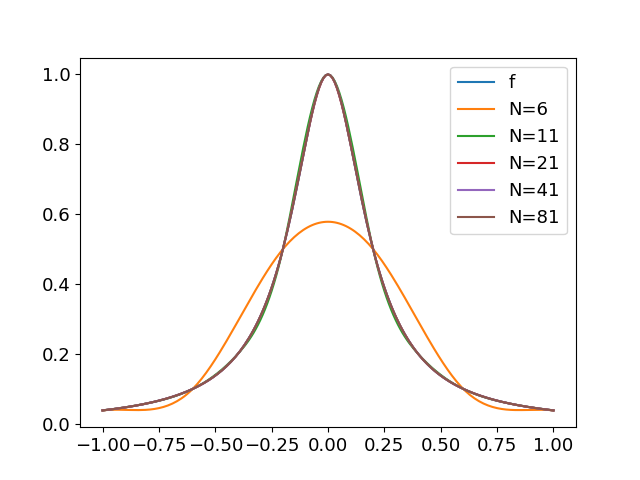
\includegraphics[scale = 0.42]{fig//ProblemA_ppForm_13.png}
  \end{minipage}
  \begin{minipage}[t]{0.5\linewidth}
    \centering
    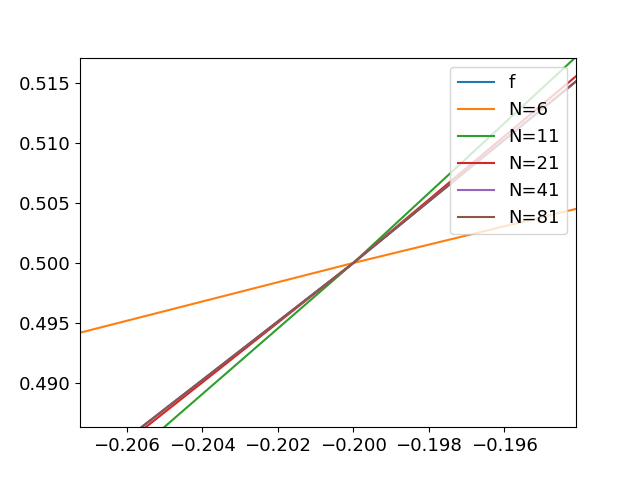
\includegraphics[scale = 0.42]{fig//ProblemA_ppForm_13_scaled.png}
  \end{minipage}
  \caption{ppForm CCS 插值图像及其局部放大图}
  \label{fig1}
\end{figure}
其次,改变\verb|A.json|中\verb|method|为2和3,分别测试cubic spline with specified second derivatives和natural cubic spline相应的插值结果,使用python作图如图。可以看出三次样条插值无论何种边界条件,都具有较好的效果,且避免了Runge现象。
\begin{figure}[H]
  \begin{minipage}[t]{0.5\linewidth}
    \centering
    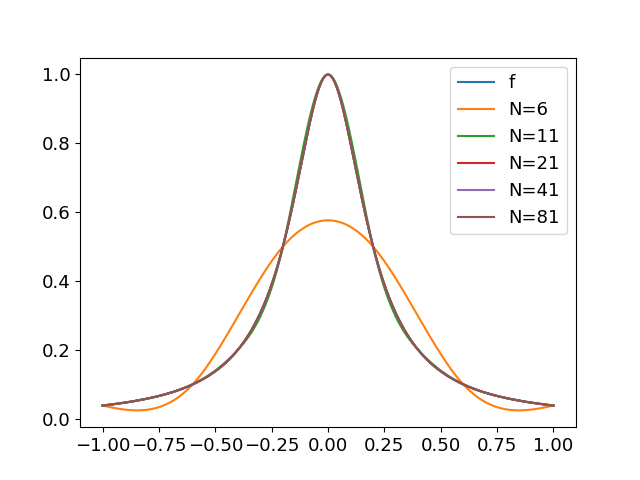
\includegraphics[scale = 0.45]{fig//ProblemA_ppForm_23.png}
    \caption{ppForm CS-SSD 插值图像}
  \end{minipage}
  \begin{minipage}[t]{0.5\linewidth}
    \centering
    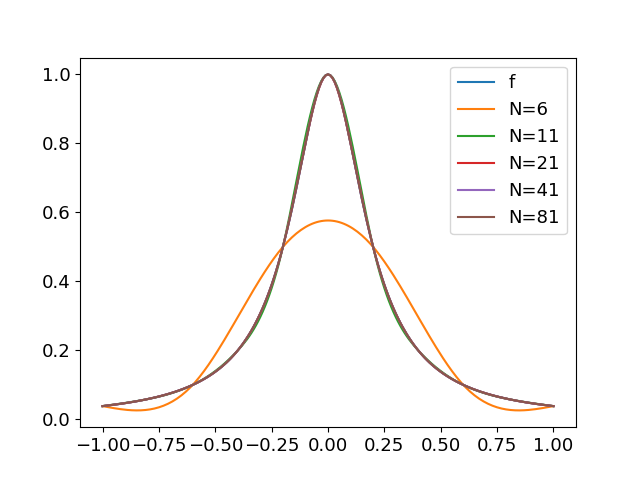
\includegraphics[scale = 0.45]{fig//ProblemA_ppForm_33.png}
    \caption{ppForm NCS 插值图像}
  \end{minipage}
  \label{fig2}
\end{figure}
最后,测试线性样条插值的结果。修改\verb|A.json|中\verb|order|为1,得到线性样条插值结果,运行程序并绘制结果图像如下。
\begin{figure}[H]
\centering
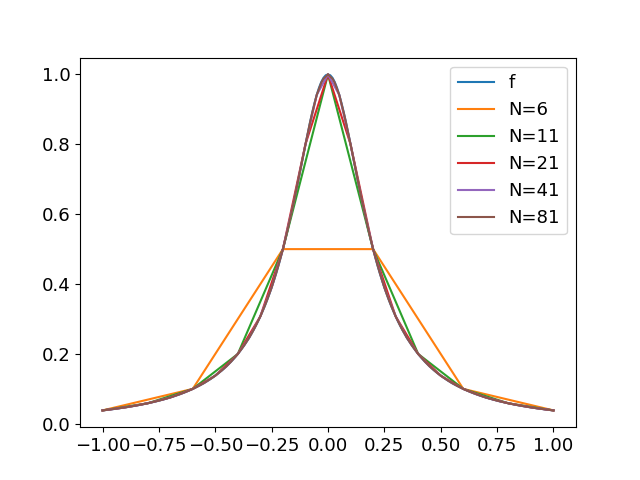
\includegraphics[scale = 0.5]{fig//ProblemA_ppForm_1.png}
\caption{ppForm 线性样条插值图像}
\label{fig3}
\end{figure}

$\bullet \;$\textbf{Bspline}:使用B样条基函数进行插值(在\verb|ProblemA.cpp|第10行修改\verb|Spline_Form|的定义即可切换ppForm和B样条之间插值方法)。与ppForm的操作方式相同,仍然绘制complete cubic spline,cubic spline with specified second derivatives,natural cubic spline和线性样条插值的结果图像,使用python展示如下所示。
\begin{figure}[H]
  \begin{minipage}[t]{0.5\linewidth}
    \centering
    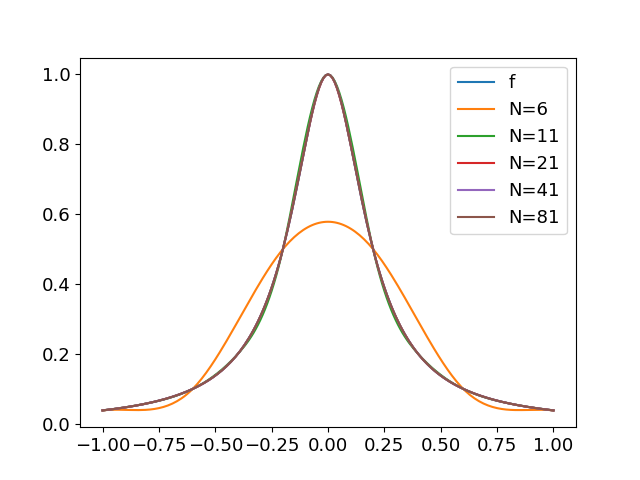
\includegraphics[scale = 0.45]{fig//ProblemA_Bspline_13.png}
    \caption{Bspline CCS 插值图像}
  \end{minipage}
  \begin{minipage}[t]{0.5\linewidth}
    \centering
    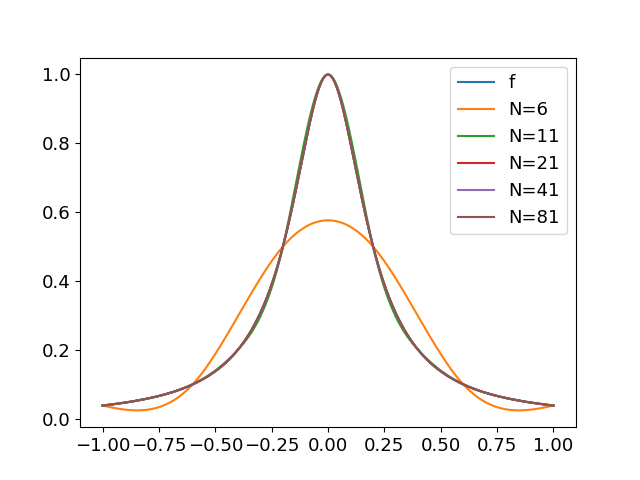
\includegraphics[scale = 0.45]{fig//ProblemA_Bspline_23.png}
    \caption{Bspline CS-SSD 插值图像}
  \end{minipage}
  \label{fig4}
\end{figure}

\begin{figure}[H]
  \begin{minipage}[t]{0.5\linewidth}
    \centering
    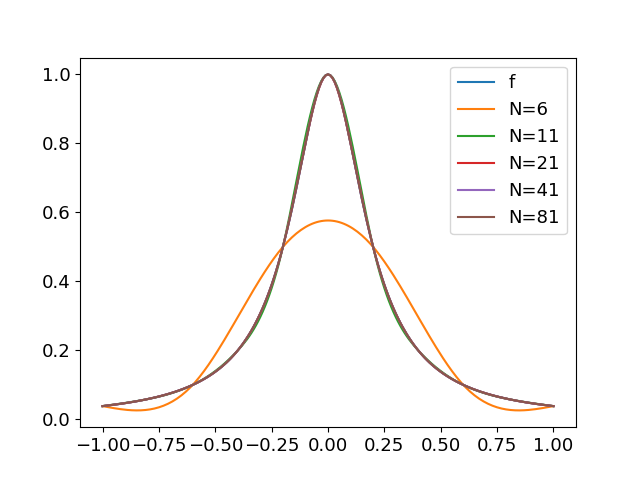
\includegraphics[scale = 0.45]{fig//ProblemA_Bspline_33.png}
    \caption{Bspline NCS 插值图像}
  \end{minipage}
  \begin{minipage}[t]{0.5\linewidth}
    \centering
    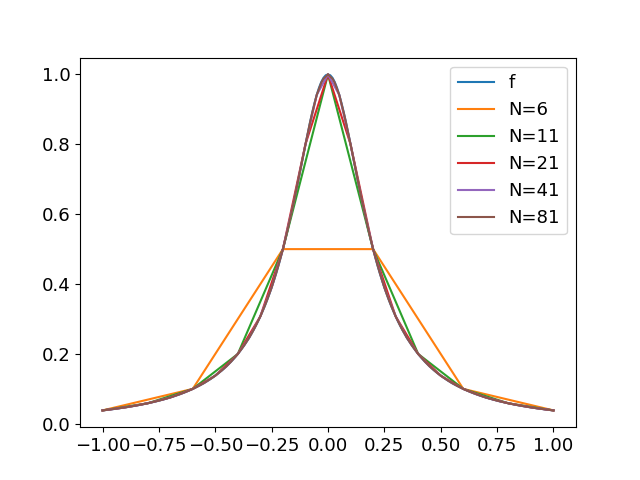
\includegraphics[scale = 0.45]{fig//ProblemA_Bspline_1.png}
    \caption{Bspline 线性样条插值图像}
  \end{minipage}
  \label{fig5}
\end{figure}
事实上,通过输出文件\verb|ProblemA_result_points.txt|的比对,可以发现ppForm和Bspline两种方法得到的结果是几乎一样的,这也从侧面说明了\verb|spline.h|中两种算法的正确性和结果的精确性。

\subsubsection{收敛阶分析}
根据题目要求,对于CCS,CS-SSD,NCS和线性样条四种情况,分别记录不同插值点个数$n$所对应的子区间中点误差最大值,输出至\verb|ProblemA_result_error.txt|中。根据上一节分析,ppForm和Bspline两种方法结果相同,故此处以ppForm为例进行分析。对于固定的$n$,对三次样条的三种边界条件的最大误差取平均值,与线性样条一并绘制最大误差和插值点个数的关系图如下。
\begin{figure}[H]
\centering
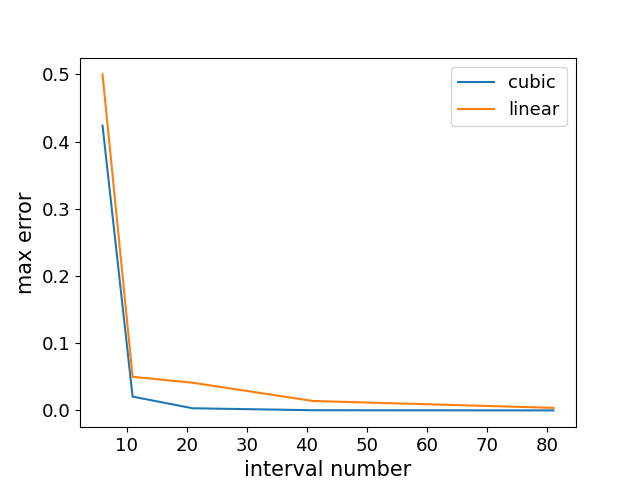
\includegraphics[scale = 0.5]{fig//ProblemA_maxerror.png}
\caption{最大插值误差和插值点个数关系图}
\label{fig6}
\end{figure}
为了对线性样条和三次样条进行收敛阶分析,我们需要对获得的最大误差进行进一步处理。首先,修改\verb|A.json|中\verb|n|为\verb|[6,11,21,41,81,161,321,641,1281]|,增加插值点个数以便观察趋势;其次,绘制最大误差序列前一项与后一项的比值,以便观察插值点个数翻倍之后最大误差缩减的比例。基于此,根据得到的数据绘制图像如图。
\begin{figure}[H]
\centering
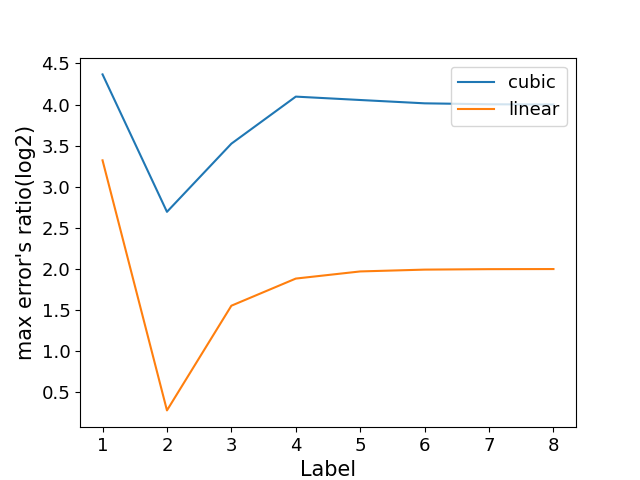
\includegraphics[scale = 0.5]{fig//ProblemA_maxerror_ratio.png}
\caption{最大插值误差比值图(以2为底)}
\label{fig7}
\end{figure}
图中Label为1对应的数值指的是$n=6$和$n=11$对应的最大误差的比值进行以2为底的对数规范化处理后的结果,以此类推。从图像中可以看出,随着插值点个数$n$的增大,三次样条的最大误差比值(以2为底)趋向于4,线性样条的最大误差比值(以2为底)趋向于2。换言之,当$n$增大一倍时,三次样条的最大误差缩小至原来的十六分之一,而线性样条的最大误差缩小至原来的四分之一。

综上所述,可以得到三次样条的收敛阶为4,线性样条的收敛阶为2。

\subsection{Problem C and Problem D}
由于问题B已经在头文件中得到更一般化的实现,故不再单独列出;问题C和问题D是针对同一个函数进行的分析,因此在本报告将其一起进行展示。另外,经向胡双助教确认,对应的二次样条只需实现线性样条进行对应分析即可,故在以下出现的二次样条部分均由线性样条进行替代。
\subsubsection{CD.json 参数说明}
以下给出\verb|CD.json|中各参数的含义说明。

$\bullet \;$ \verb|point_1|:三次Bspline插值点。在误差分析的补充中需要修改。

$\bullet \;$ \verb|point_2|:线性Bspline插值点。本题中无需修改。

$\bullet \;$ \verb|output_point|:误差函数需要输出值的点。本题中无需修改。
\subsubsection{插值结果展示}
对函数
\begin{equation}
    f(x) = \frac{1}{1+x^2}
\end{equation}
分别根据\verb|CD.json|中给定的插值点使用三次B样条插值(根据题目要求,使用complete cubic spline)和线性B样条插值,得到结果输出至\verb|ProblemC_result_points.txt|,利用python绘制结果图像和实际函数图像如图所示。
\begin{figure}[H]
\centering
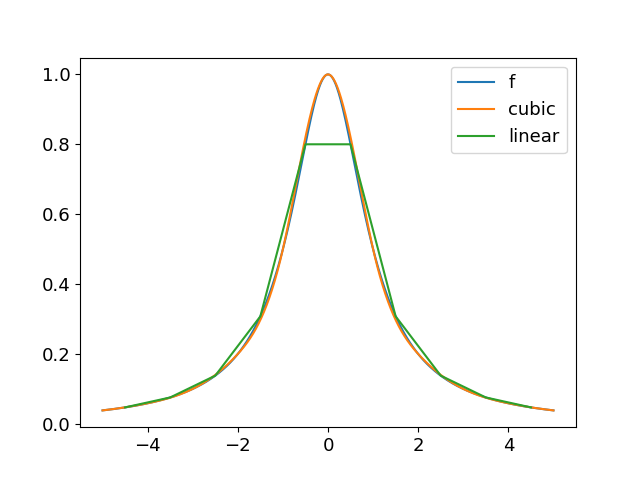
\includegraphics[scale = 0.5]{fig//ProblemC_Bspline_1&3.png}
\caption{Bspline CCS和线性样条插值图像}
\label{fig8}
\end{figure}
从图像可以看出,三次样条插值相较于线性样条插值,对于$f$的拟合结果更加精确。具体的误差分析将在下一节中展开叙述。

\subsubsection{误差展示和分析}
对于C题中得到的两个插值函数$S$,分别计算误差函数$E_S(x) = |S(x)-f(x)|$,将结果采样输出至\verb|ProblemD_result_errorpoints.txt|中,并基于此绘图如下。
\begin{figure}[H]
\centering
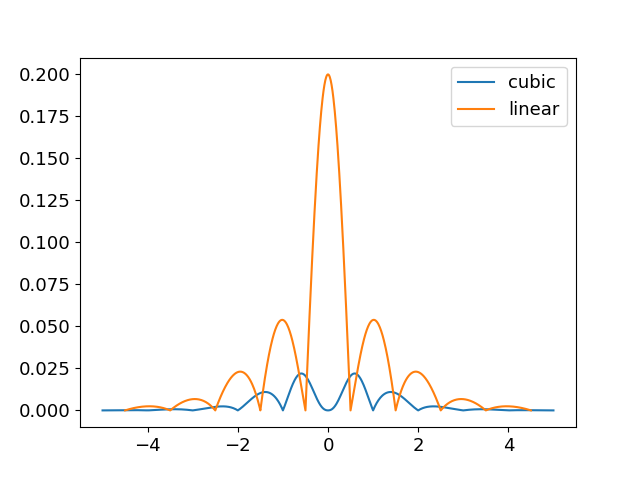
\includegraphics[scale = 0.5]{fig//ProblemD_errorfunction.png}
\caption{Bspline CCS和线性样条插值误差图像}
\label{fig9}
\end{figure}
从图像中可以清晰地看出三次样条的误差要小于线性样条插值,故三次Bspline的结果更加精确。进一步,根据题目要求,输出三次样条和线性样条在$x=-3.5,-3,-0.5,0,0.5,3,3.5$处的误差函数值于\verb|ProblemD_result_error.txt|,展示如下:
\begin{shaded}
\begin{verbatim}
Error values of cubic spline at required points
0.000669568, 0, 0.0205289, 0, 0.0205289, 0, 0.000669568
Error values of linear spline at required points
0, 0.00670137, 0, 0.2, 0, 0.00670137, 0
\end{verbatim}
\end{shaded}
可以发现,部分$x$处的误差为0。仔细观察,发现误差接近0对应的$x$恰巧是插值结点,它们的误差很小是因为样条插值要求节点处的插值函数值等于原函数的值,因此在求解精确度高的条件下,插值结点的误差应当接近0。这也可以从图像中看出:误差函数在插值结点的误差很小,而在每一个插值子区间的中点处取到极大值。

\subsubsection{误差分析补充}
第四章理论题\uppercase\expandafter{\romannumeral13}中提到,如果某两个插值点间距远小于其他插值点,会造成结果不准确。在此给出对其的验证。

首先将\verb|CD.json|中\verb|point_1|修改为
\begin{shaded}
\begin{verbatim}
"point_1" : [-5,-3.000001,-2.999999,-1,1,3,5]
\end{verbatim}
\end{shaded}
显然,$-3$附近的两个插值点的间距要远小于其余各插值点的间距。然后再扩大该插值点间距,将\verb|point_1|修改(作为对照)为
\begin{shaded}
\begin{verbatim}
"point_1" : [-5,-3.1,-2.9,-1,1,3,5]
\end{verbatim}
\end{shaded}
对于以上两组插值点,分别计算其误差函数$E_S(x)$,绘制其在$[-3,-1]$区间附近的放大图像如下。
\begin{figure}[H]
\centering
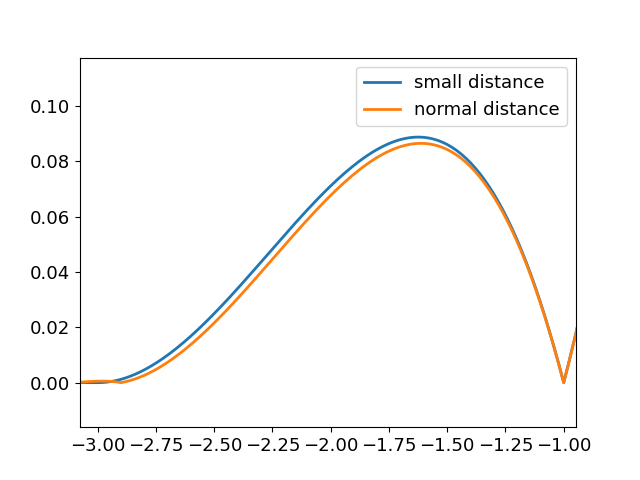
\includegraphics[scale = 0.5]{fig//ProblemD_errorfunction_plug.png}
\caption{不同插值点间距对应插值误差对比图(局部)}
\label{fig9}
\end{figure}
由图像可知,若某两点的间距远小于其他插值点间距时,对应的插值误差会略有增大但不明显。插值误差会略有增大验证了第四章对应理论的正确性,而误差增大不明显可能是因为算法和计算的精度都相对较高。

\subsection{Problem E}
本题中,对于心形曲线
\begin{equation}
    x^2+(\frac{3}{2}y-\sqrt{|x|})^2=3,
\end{equation}
程序将根据不同的插值点个数,分别使用三次和线性样条进行曲线插值,并对结果给出可视化的展示。

\subsubsection{E.json 参数说明}
以下给出\verb|E.json|中各参数的含义说明。

$\bullet \;$ \verb|n|:插值点个数表。本题中无需修改。

$\bullet \;$ \verb|order|:样条阶数。输入1或3,分别代表线性和三次样条。

$\bullet \;$ \verb|spline_form|:插值方式。输入\verb|"Bspline"|或者\verb|"PP"|,分别代表Bspline插值法和ppForm插值。本报告的结果\textbf{默认}使用Bspline插值,如需改成ppForm可进行相应修改,也可得到相同的结果。

\subsubsection{思考题}
$\bullet \;$ \textbf{样条组数}:事实上,\verb|spline.h|可以自动实现任意维度的曲线样条插值。对于本题的而言,心形曲线是二维的,因此需要两组样条进行插值。

$\bullet \;$ \textbf{边界条件}:对于线性样条,无需边界条件;对于三次样条,我认为natural cubic spline的边界条件是最合适的。曲线插值的自变量是cumulative chordal lengths,而根据定义,cumulative chordal lengths依赖于插值点的选取(且本身就是离散形式的),因此一般是无法给出待插值函数的解析表达式,当然也无法给出其在某一点的一阶导或者二阶导数的值。从这个角度而言,选择CCS或者CS-SSD作为边界条件是不妥的,而NCS规定在插值区间端点处的二阶导数为0,既具有其实际意义,又避免了导数的计算,因此相对更为合理。

$\bullet \;$ \textbf{插值点选取}:本程序采用
\begin{equation}
    (0,\pm\frac{2}{3}\sqrt{3}),\quad(\pm\sqrt{3},\frac{2}{3}\sqrt[4]{3})
\end{equation}
这四个点作为characteristic points,对于其他插值点,程序采用顺时针方向,根据$x$坐标均匀间隔依次分配插值点。

\subsubsection{插值结果展示}
$\bullet \;$\textbf{三次样条}:结合上述分析,设定\verb|E.json|中参数\verb|order|为3,即可分别根据插值点个数$n=10,40,160$进行心形曲线三次样条插值,得到结果输出至\verb|ProblemE_result_points.txt|,后利用python绘制插值图像及其对比图如下所示。
\begin{figure}[H]
  \begin{minipage}[t]{0.5\linewidth}
    \centering
    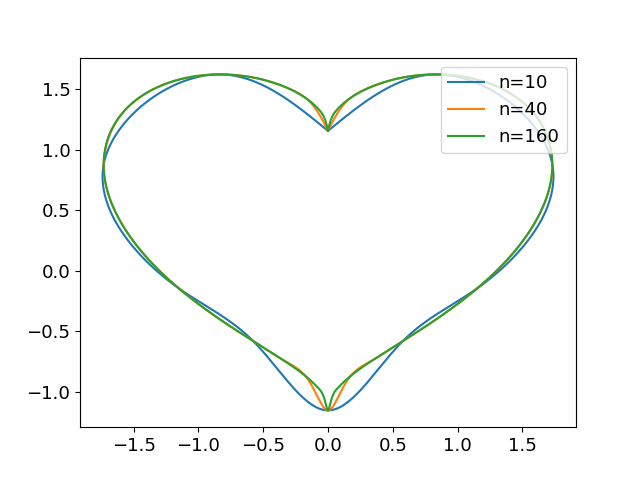
\includegraphics[scale = 0.45]{fig//ProblemE_heartplotx3.png}
    \caption{三次样条插值结果对比图}
  \end{minipage}
  \begin{minipage}[t]{0.5\linewidth}
    \centering
    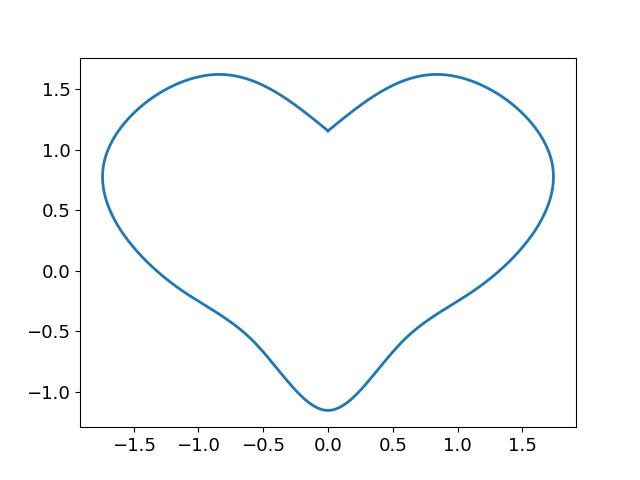
\includegraphics[scale = 0.45]{fig//ProblemE_heartplot_10.png}
    \caption{三次样条插值结果($n=10$)}
  \end{minipage}
  \label{fig10}
\end{figure}
\begin{figure}[H]
  \begin{minipage}[t]{0.5\linewidth}
    \centering
    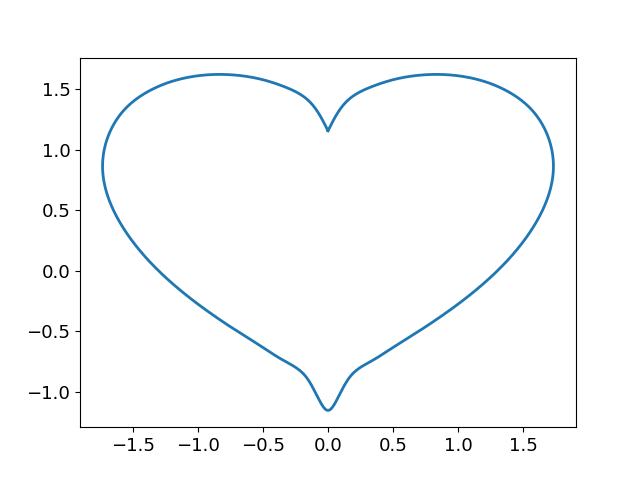
\includegraphics[scale = 0.45]{fig//ProblemE_heartplot_40.png}
    \caption{三次样条插值结果($n=40$)}
  \end{minipage}
  \begin{minipage}[t]{0.5\linewidth}
    \centering
    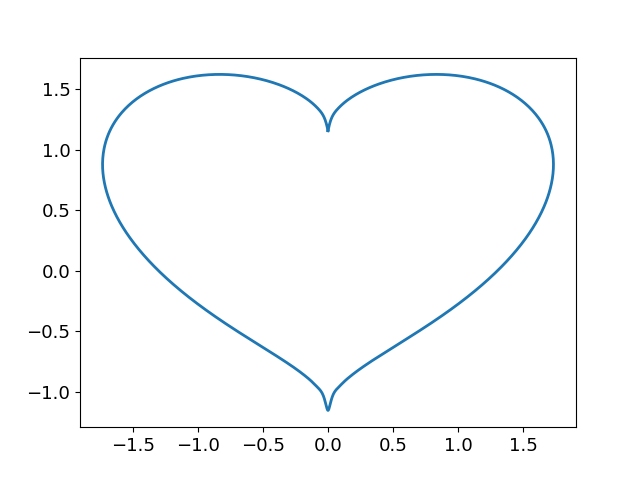
\includegraphics[scale = 0.45]{fig//ProblemE_heartplot_160.png}
    \caption{三次样条插值结果($n=160$)}
  \end{minipage}
  \label{fig11}
\end{figure}
可以看出,插值曲线的轮廓是较为光滑的,并且随着插值点个数$n$的增大,曲线三次样条插值结果与心形越来越接近,同时可以很好地反映出心形曲线的轮廓特征。这也从侧面说明了选择characteristic points的合理性。

$\bullet \;$\textbf{线性样条}:同样地,修改\verb|E.json|中参数\verb|order|为1后,即可分别根据插值点个数$n=10,40,160$进行心形曲线线性样条插值,得到结果输出至\verb|ProblemE_result_points.txt|,后利用python绘制插值图像及其对比图如下所示。
\begin{figure}[H]
  \begin{minipage}[t]{0.5\linewidth}
    \centering
    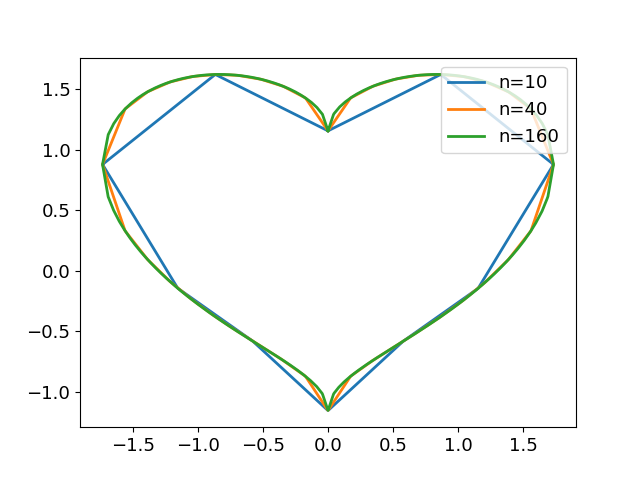
\includegraphics[scale = 0.45]{fig//ProblemE_heartplotx3_linear.png}
    \caption{线性样条插值结果对比图}
  \end{minipage}
  \begin{minipage}[t]{0.5\linewidth}
    \centering
    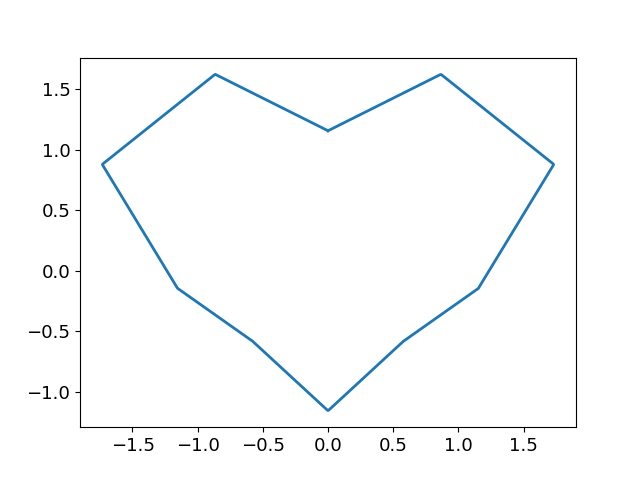
\includegraphics[scale = 0.45]{fig//ProblemE_heartplot_10_linear.png}
    \caption{线性样条插值结果($n=10$)}
  \end{minipage}
  \label{fig12}
\end{figure}
\begin{figure}[H]
  \begin{minipage}[t]{0.5\linewidth}
    \centering
    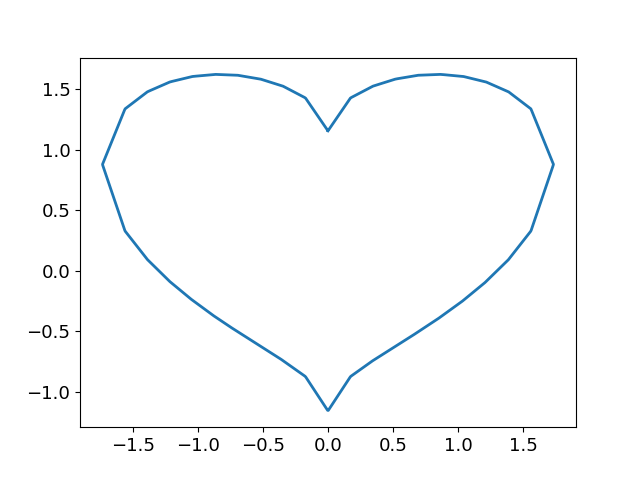
\includegraphics[scale = 0.45]{fig//ProblemE_heartplot_40_linear.png}
    \caption{线性样条插值结果($n=40$)}
  \end{minipage}
  \begin{minipage}[t]{0.5\linewidth}
    \centering
    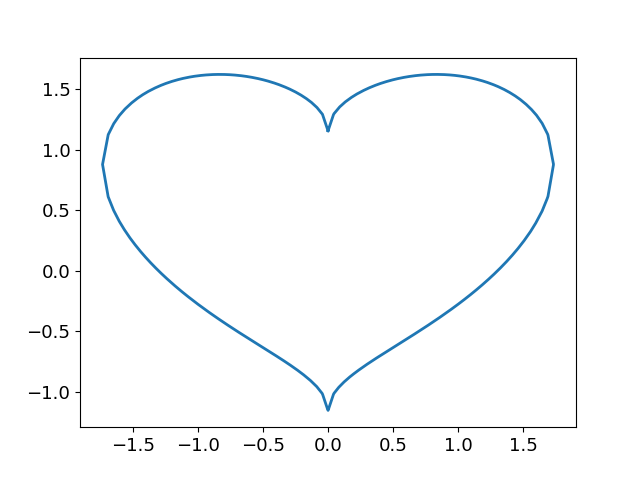
\includegraphics[scale = 0.45]{fig//ProblemE_heartplot_160_linear.png}
    \caption{线性样条插值结果($n=160$)}
  \end{minipage}
  \label{fig13}
\end{figure}
对比线性样条和三次样条曲线插值的图像,可以较明显地看出三次样条的拟合结果更加光滑且精确。
\end{sloppypar}
\end{document}
